\documentclass[12pt,a4paper]{book}
\usepackage[utf8]{inputenc}%acepta tildes, simbolos y eñes
\usepackage{color}
%\usepackage{minted}%pip install pygments
%https://ondiz.github.io/cursoLatex/Contenido/11.Codigo.html.
%https://tex.stackexchange.com/questions/99475/how-to-invoke-latex-with-the-shell-escape-flag-in-texstudio-former-texmakerx
\usepackage{minted}
\usepackage{listings}
\usepackage[spanish]{babel}%%permite escribir algunas estructuras en español, como la fecha actual en el sistema
\usepackage{amsmath}
\usepackage{amsfonts}
\usepackage{amssymb}
\usepackage{caption}
\usepackage{subcaption}
\usepackage{xcolor}
\usepackage{array,longtable}
\usepackage{float}%para usar el posicionador H, permitiendo que la tabla aparezca en la posicion del codigo fuente
\definecolor{azul}{rgb}{0.17, 0.40, 0.69}%creacion de mi propio color azul
\usepackage{setspace}%permite hacer un interlineado
\usepackage{lipsum}%para agregar chapters (capitulos)
\usepackage{graphicx}%permite insertar graficas desde el exterior
\usepackage[left=2.0cm,right=2.0cm,top=2.0cm,bottom=2.0cm]{geometry}%margenes a la izquierda,derecha,arriba y abajo
\usepackage{wrapfig}%para mezclar imagenes y texto

\usepackage{tabularx}
\author{Cristian Hernández Resendiz}
\title{Logística}
\begin{document}
	\begin{titlepage}
	\begin{center}
		{\huge \textbf{Instituto Politécnico Nacional}}\\
		\vspace{1cm}%%espacio vertical de 1 cm
		{\large \textbf{"La técnica al servicio de la patria"}}\\
		\vspace{3mm}
		\begin{figure}[h]
			\centering%%centramos nuestra figura
			
\includegraphics[height=6cm]{logoIPN.PNG}
		\end{figure}
		\vspace{3mm}
		{\LARGE \textbf{Escuela Superior de Cómputo}}\\
		\vspace{3mm}
		\textcolor{azul}{\rule{\linewidth}{0.75mm}}%%esta linea describe que vamos a dibujar una linea de color azul con un grosor de 0.75
		\\
		\begin{spacing}{1.5}
			{\LARGE \textsc{Autómata celular: el juego de la vida}}
		\end{spacing}
		\textcolor{azul}{\rule{\linewidth}{0.75mm}}\\
		\vspace{5mm}
		{\large \textbf{Alumno: Cristian Hernández Resendiz}}\\
		\vspace{2mm
		{\large \textbf{Optativa: Computing selected topics}}\\
		\vspace{2mm}}
		{\large \textbf{Materia: Complex systems}}\\
		\vspace{2mm}
		{\large \textbf{Profesor: Genaro Juarez Martínez}}\\
		\vspace{2mm}
		{\large \textbf{Grupo: 3CM9}}\\
		\vspace{2mm}
		{\large \textbf{Boleta: 2016602153}}\\
	\end{center}
\end{titlepage}

%textbf es texto en negritas
%textsc es para dar estilo a la letra
%rule es para dibujar una linea
	\tableofcontents%inserta un indice
	\chapter{Introducción}
	%
	Un ecosistema, o el medioambiente en general, son sistemas complejos. Las organizaciones y estructuras
	humanas (económicas, sociales, políticas, etc ) son aún más complejas.
	Cualquier análisis o estudio territorial, a la escala que sea, cualquier plan de desarrollo, ya sea urbanístico o
	económico, cualquier decisión política y toda intervención en un ámbito social determinado incide en un medio
	muy dinámico y cambiante; muchas veces autónomo en su evolución. Actuaciones que persiguen un beneficio o
	la mejora de una situación dada pueden fácilmente tener efectos inesperados y provocar a la postre un efecto
	contrario.
	El estudio de un sistema de estas características es hoy en día un reto para cualquier disciplina científica. Los
	economistas por su lado, los urbanistas por otro; los sociólogos en su esfera o los politólogos en la suya, todos
	se enfrentan a la dificultad de 'manejar' adecuadamente estas estructuras dinámicas. Más si cabe cuando la
	meta es pronosticar la evolución futura del sistema en cuestión. Y de ello dependen muchos intereses y a veces
	hasta muchas vidas.
	La naturaleza impredecible de estos sistemas se asume en general como una característica intrínseca y propia
	y lo que es peor, inevitable. Se trate de la Bolsa, de la economía local o internacional, de la evolución de la moda,
	de la competencia industrial en los mercados, de la respuesta social a fenómenos culturales o del estudio de los
	índices de gobernanza de un país, resulta escasa la precisión en la descripción de la situación en el presente
	mientras que se convierte en un arte adivinatorio la predicción de su evolución futura.
	Para poder diagnosticar correctamente un sistema de este tipo habría que recopilar y luego integrar una
	cantidad de datos tan inmensa que los ordenadores que disponemos en la actualidad se quedan cortos. Pero
	el problema no es sólo ese. Suponiendo que pudieramos disponer de la tecnología adecuada aún quedaría por
	solucionar otro asunto. Un sistema complejo es tan dinámico que cambia continuamente. Por lo tanto, los datos
	que se obtuvieron ayer y que se analizan hoy igual ya no tienen nada que ver con la realidad de mañana.
	Hasta ahora la estrategia de aproximación al estudio de lo complejo se basa en el cálculo estadístico. Se
	seleccionan una serie limitada de variables del sistema, las que a priori se considera que más influyen en los
	procesos internos de la estructura y se trabaja con ellas estableciendo correlaciones y sacando así conclusiones.
	Muchas veces este modo de aproximación funciona bien y permite obtener una visión muy realista de la
	situación y, a veces, hasta sirve para anticiparse a los cambios que se producen. Sin embargo también ocurre
	con demasiada frecuencia que cuando el investigador cree controlar todas las variables importantes, aparece
	una nueva e inesperada que ha adquirido un protagonismo imprevisto en el funcionamiento del sistema y por
	extensión, en su evolución. Por ello, estos modos de aproximación, estas técnicas de estudio, tienen un valor
	muy relativo y una utilidad bastante limitada.
	El ejemplo más ilustrativo de un sistema complejo es un organismo biológico. Una célula, un órgano, una
	planta o un animal responden a este patrón. Pero así mismo lo es la estructura social en la que se organizan
	las poblaciones de animales como termitas, hormigas, abejas, una familia de leones o una manada de antílopes.
	Lo es también una comunidad de seres vivos, animales y vegetales, que comparten un hábitat en cualquier
	ecosistema en general. Y lo es así mismo un bioma, a una escala mucho más amplia y referida a las condiciones
	climáticas de una zona del planeta. Cada uno de ellos, a su nivel, actúa como una unidad autónoma, como un
	organismo individual. Dispone de un 'dentro' organizado y de un 'afuera' con el que interactúa.
	Aunque pueda parecer a primera vista que el límite de un sistema esta bien definido, lo que nos resulta casi
	evidente en el caso de una célula, de un órgano, de una planta o de un animal, no podemos olvidar que el sistema
	no existe sin su medio exterior con el cual intercambia constantemente energía y materia. La respiración y la
	alimentación son buena prueba de ello.
	Por otra parte, un individuo siempre es parte constituyente de otra individualidad superior. Y a su vez,
	ese mismo individuo esta compuesto de partes constituyentes que son individualidades a su vez, en una
	escala inferior. Esto crea una estructura jerárquica de sistemas que engloban otros subsistemas en una sucesión
	interminable.
	%
	Este es el caso de la célula que visualizamos perfectamente como un ente individual y autónomo. Sin embargo,
	esa misma célula, integrada en un tejido y tal vez en un órgano, es parte de un ser superior. Es un simple
	ladrillo de la arquitectura de ese ser superior. Pero la célula no es indivisible. Todo lo contrario, ella misma
	esta 'fabricada' por componentes menores que pueden describirse en una escala descendente. Así, podemos
	establecer una primera división en núcleo, citoplasma y membrana y luego podemos ir descendiendo al nivel de
	los organélos celulares y de allí a la escala de las macromoléculas.
	A su vez, el ser superior de esa célula, ya sea una planta o un animal, comparte su existencia con sus
	congéneres. En un espacio común, en un trozo de terreno específico, interaccionan entre todos ellos y crean una
	unidad superior dotada de 'individualidad' propia. Es la manada o la bandada o la familia o la colmena, etc.
	Dada esta idea, a continuación se presenta un juego que simula el movimiento de células dentro de un espacio
	bidimensional; se trata del juego de la vida.
	%
	\chapter{Desarrollo}
	\section{El juego de la vida, un autómata celular}
	%
	En el año 1970, el matemático inglés John Horton Conway creó un juego matemático de simulación que
	consistía en un universo cuadriculado donde es posible determinar un estado inicial y luego hacerlo correr para
	observar su evolución. Lo llamó 'el Juego de la Vida 2' es en realidad un autómata celular. Esto es, un modelo
	matemático para un sistema dinámico que va evolucionando en pasos discretos.
	El juego es un autómata celular bidimensional en el cual cada celda (célula) puede estar en uno de los
	dos estados posibles, viva o muerta. Partiendo de un estado inicial, la simulación va haciendo evolucionar al
	autómata en base a unas sencillas funciones de transición. Una célula va a estar en un estado concreto, el cual
	sera determinado únicamente del estado inmediatamente anterior de las células vecinas y el de la propia
	célula.
	
	%
	\subsection{Reglas}
	El conjunto de reglas básicas que propuso Conway son las siguientes:
	\\
	\begin{itemize}
		\item Una célula muerta con exactamente 3 células vecinas vivas 'nace' (es decir, al turno siguiente estará viva).
		\item Una célula viva con 2 o 3 células vecinas vivas sigue viva, en otro caso muere (por 'soledad' o 'superpoblación').
	\end{itemize}

Cada célula viva o muerta en el espacio bidimensional se rige en sus 8 células vecinas cercanas de la siguiente
manera.
%
\begin{figure}[H]
	\centering
	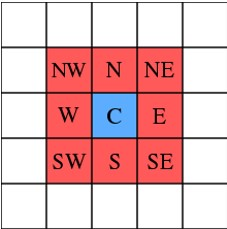
\includegraphics[width=0.2\textwidth]{imagen1PC}
	\caption{Vecindad de Moore}
\end{figure}
%
La célula C  esta rodeada de 8 celdas de color rojo. Estas últimas son células que pueden estar vivas o muertas. Todas las células en el espacio bidimensional determinan su estado mediante sus 8 vecinas cercanas, siendo estas vivas o muertas en ese momento.

	\subsection{Patrones}
	Un patrón es una configuración de células que permanecen vivas en un momento determinado. Existen
	básicamente 3 clases de patrones en el juego de la vida de Conway.
	\begin{itemize}
		\item Patrones estáticos: Un conjunto de células vivas que se mantiene estático, sin que se produzcan nuevos
		nacimientos o muertes.
		\begin{figure}[H]
			\centering
			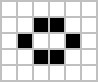
\includegraphics[width=0.2\textwidth]{imagen2PC}
			\caption{Patrones estáticos}
		\end{figure}
		\item Patrones recurrentes: Un conjunto de células vivas que no se mueve por el mundo, pero que no es estático,
		ya que se producen nacimientos y muertes, produciendo transiciones que se repiten continuamente.
		\begin{figure}[H]
			\centering
			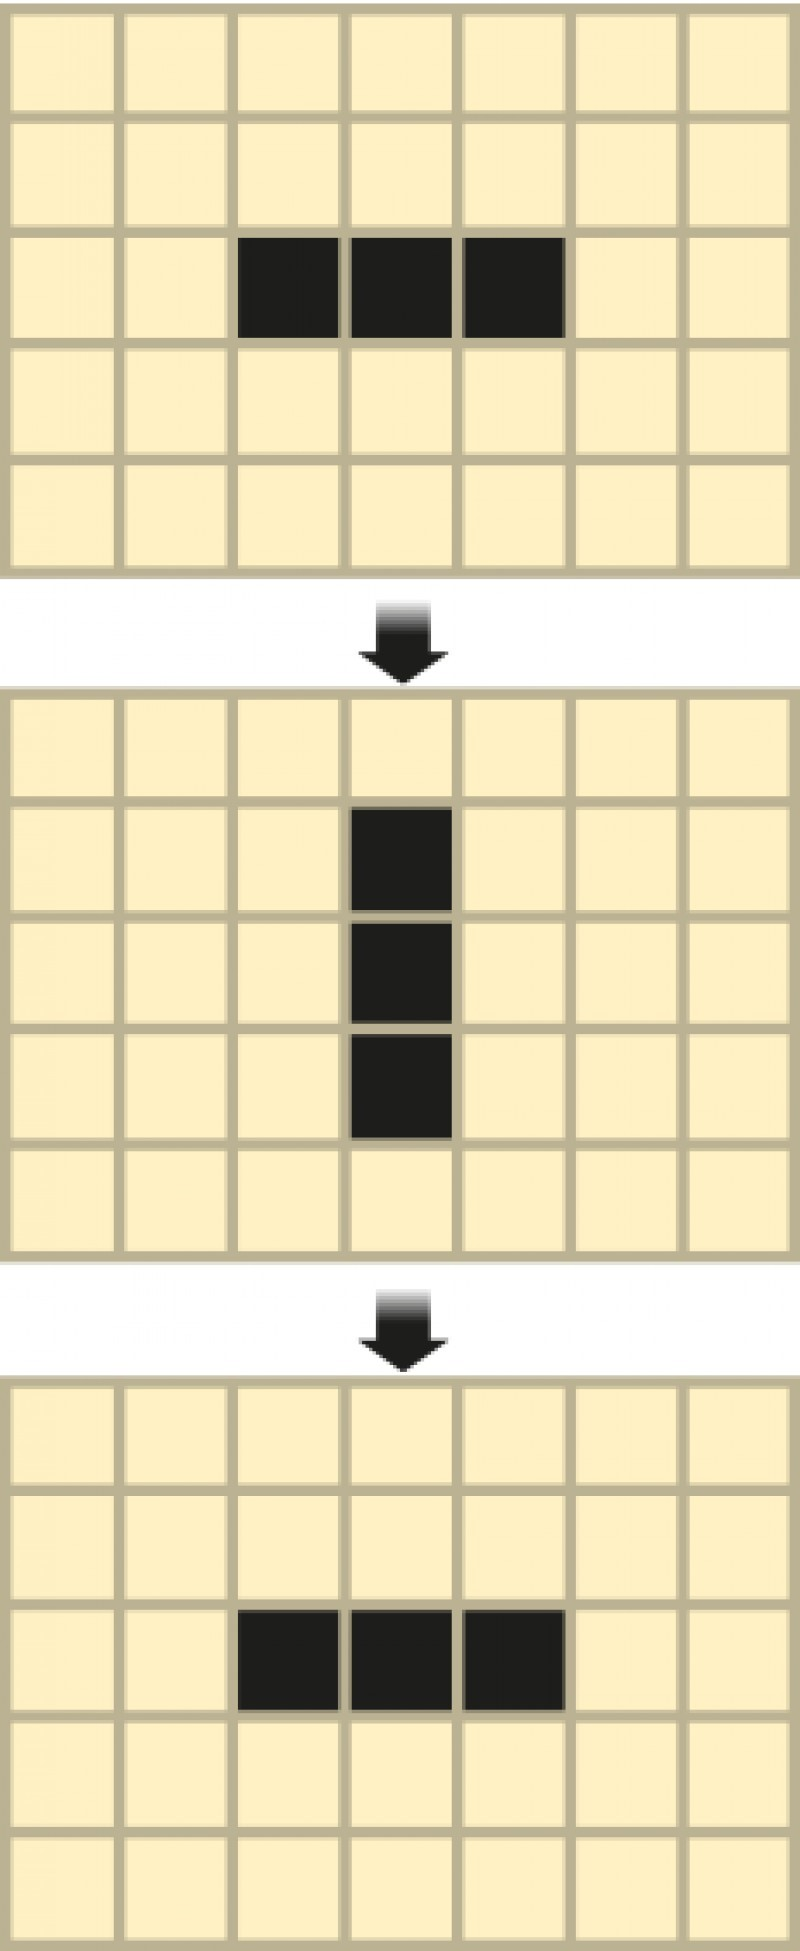
\includegraphics[width=0.2\textwidth]{imagen3PC}
			\caption{Patrones recurrentes}
		\end{figure}
		\item Patrones que se trasladan: Un conjunto de células vivas que permanece con la misma forma, pero que se
		desplaza por el tablero.
		\begin{figure}[H]
			\centering
			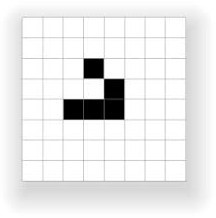
\includegraphics[width=0.2\textwidth]{imagen4PC}
			\caption{Patrones en traslación}
		\end{figure}
	\end{itemize}
	\section{Atractores, caos y complejidad}
	%
	Las condiciones para que un sistema sea no caótico (lineal) son que: 1) si situamos un objeto en una posición determinada, podremos calcular con exactitud y de forma sencilla en que posición se encontrará al cabo de cierto tiempo; 2) si situamos dos objetos en posiciones iniciales cercanas, al cabo del tiempo dichos objetos permanecerán más o menos cercanos, ya que sobre ellos actuarán fuerzas de parecida magnitud. En el análisis de los sistemas complejos, la base del análisis es lo nolineal. Se habla de sistemas lineales cuando estos sistemas son predecibles, previsibles. Un sistema caótico es, sin duda, un sistema más difícil de tratar, ya que debido a su imprevisibilidad siempre tiene alguna sorpresa que ofrecer (Nicholls 1998) . Si un sistema dinámico es caótico, tiene un componente de impredicibilidad, un componente de irreducibilidad, pero aun así tiene un tercer componente de regularidad (Upm 1998). Un caos totalmente aleatorio conlleva la irregularidad en su comportamiento, y el análisis científico actual ha avanzado poco en su conocimiento.

Ha quedado señalado que en la Tcaos actual existen dos enfoques básicos para entender el desorden de los sistemas: el “enfoque de las estructuras disipativas”, y el “enfoque de los atractores”. En el primero, el caos se considera como el precursor y socio del orden y no como su opuesto. Aquí se centra la atención en el surgimiento espontáneo de “autoorganizaciones” que emergen del caos, o, según la terminología del campo, en las “estructuras disipativas” que surgen en sistemas fuera de equilibrio, cuando la producción de entropía es alta. La comprensión de que los sistemas ricos en entropía facilitan en vez de impedir la auto-organización ha sido una coyuntura decisiva para la revaluación contemporánea del caos.

El segundo enfoque destaca el orden oculto que existe dentro de los sistemas caóticos. Usado de este modo, el término “caos” difiere de la total aleatoriedad, porque se puede demostrar que contiene estructuras profundamente codificadas, llamadas “atractores extraños”. Mientras que los sistemas verdaderamente aleatorios no muestran un esquema discernible cuando se les organiza en el espacio de fase, los sistemas caóticos se concentran en una región limitada y trazan modelos complejos dentro de ella (Hayles 1998: 29).

El enfoque de las “estructuras disipativas” permite entender que el conjunto de los diversos sistemas naturales, biológicos y humanos (supersistema), generan durante su convivencia intercambios de energía, recursos o informaciones, lo que da origen a la entropía. Esta, en lugar de degenerar o perderse, es aprovechada por algunos sistemas para revitalizarse, o transformarse, lo cual puede dar origen, o recrear, nuevas estructuras (sistemas). La naturaleza emplea el caos en forma constructiva. Al amplificar las pequeñas fluctuaciones provee sistemas que permiten el acceso a la creatividad. Los sistemas complejos pueden generar anticaos, es decir, un sistema desordenado que “cristaliza” en orden. El caos puede proporcionar los medios para estructurar los cambios azarosos, ofreciendo la posibilidad de poner la diversificación bajo el control de la evolución (Schifter 1996: 100-103). De esta manera, el supersistema se autorganiza a partir del caos.

Por su parte, el enfoque de los “atractores” proporciona herramientas para entender o delimitar (“medir”) dicho caos. Atractor es el término técnico para la figura o trayectoria básica del estado final al que tiende el sistema (Gleick 1987:121-153). Por ejemplo, si se pone una canica en un embudo, acabará siempre en el agujero, independientemente de la pared del embudo donde se haya colocado inicialmente. El agujero del embudo sería el atractor del sistema. Un gran atractor contiene todos los posibles estados finales de un sistema dinámico, una especie de metaembudo. El ejemplo clásico es el clima, el cual sería el gran atractor de la meteorología (Navaltropo 1998). La complejidad de este atractor ha hecho que se le denomine como extraño atractor.

Es importante apreciar que los patrones de fase espacial de un sistema caótico nunca coinciden. Si esto ocurriera, el sistema se transformaría en periódico. Un atractor de un sistema caótico de las ciencias duras es una maraña de trayectorias, una “turbulencia”. Superficialmente, el atractor parece estar completamente desorganizado. Sin embargo, una observación más cuidadosa de la fase espacial revela que el atractor está organizado pero de una manera no convencional. A diferencia de las ciencias duras, en las “ciencias blandas” los atractores tienden a ser “elementos”, “factores”, “cuellos de botella” o “causas” que originan desórdenes en la sociedad, su economía, cultura o política. En las regiones los atractores son "elementos" generadores de entropía (activa o inactiva) (Briggs 1994: 19-23). Por consiguiente, los “atractores regionales” generan a la vez bienestar y caos en las regiones, y son resultado de la acumulación de experiencias, situaciones, conocimientos y actitudes resultado de la interacción de la sociedad, la economía, la cultura, la ecología y el territorio de las propias regiones. Se convierten en referentes que en ocasiones repentinamente son activados por situaciones que se asemejan a las experiencias precedentes: están siempre presentes en espera de ser puestos en operación por la propia interacción de las regiones. A través de los atractores, las regiones confirman su carácter complejo, cambiante, su comportamiento no lineal, oscilante entre el orden y el caos, entre el bienestar y el desorden.
\\
En un sistema caótico complejo como el de la región es posible la existencia de atractores múltiples (Nicholls y Tagarev 1998). Esto significa que los sistemas caóticos pueden tener diversos niveles de estabilidad-inestabilidad cuando operan a favor del bienestar o del desorden. El clima de la tierra es un buen ejemplo de esta forma de comportamiento, pue se estima que el clima actual sufre comportamientos inesperados, pasando de una situación a otra. En las regiones, los cambios pueden deberse a la presencia de diversos atractores, algunos básicos, como la pobreza o el desempleo, cuya presencia afecta la estructura del sistema; otros intermedios, como la aparición de un orden social alternativo, los cuales generan cambios parciales en los sistemas sociales; y también la existencia de atractores profundos como la destrucción cultural o ecológica, los cuales tienden a ocasionar el cambio radical del sistema. En estos casos el caos se genera debido a la activación de un atractor.
	
	%
		\begin{figure}[H]
		\centering
		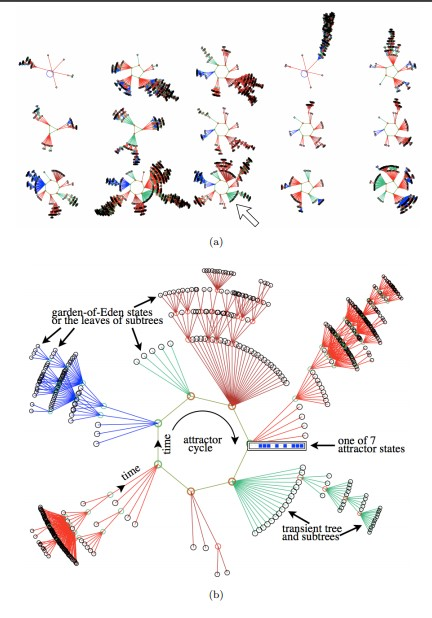
\includegraphics[width=0.9\textwidth]{atractoresSistemasDinamicos}
		\caption{En (a) se ilustra el campo del conjunto de atracción de una red
booleana aleatoria (RBN), En (b) se presenta en detalle un conjunto de atracción, como configuraciones de bits (flecha de arriba indicada en (a)) con 604 estados de los cuales 523 son hojas y el atractor es de periodo igual a 7. La
dirección del tiempo es hacia dentro del atractor y con orientación al sentido de
las manecillas del reloj.
}
	\end{figure}
	
	
	\section{Descripción del software de aplicación}
	Se ha realizado una versión del juego de la vida de Conway en un universo plano empleando el lenguaje de programación interpretado llamado \textbf{python}. Esta versión cuenta con las siguientes funcionalidades:
	\begin{itemize}
		\item \textbf{Control del juego:} Es posible pausar y reproducir el juego cuando el usuario lo desee.
		\item \textbf{Cambiar el color de las células:} El programa permite cambiar el color de las células vivas y muertas que están en el espacio celular de evolución
		\item \textbf{Cambiar el tamaño de la célula:} La célula puede tener tamaño de hasta 10 px (pixeles).
		\item \textbf{Cargar configuraciones: } Esta función le permite al usuario cargar patrones de células vivas guardados en archivos .npy
		\item \textbf{Guardar configuraciones:}  El programa tiene un módulo para guardar patrones de células vivas que estén en el espacio celular plano
		\item \textbf{Ver gráfica de la densidad de células vivas: }En este punto, el usuario tiene la opción de visualizar las células vivas que han estado en cada fase de evolución. Estos datos están expresados en una gráfica.
		\item \textbf{Añadir y borrar células en el espacio celular:} Cuando el usuario de un click izquierdo o derecho sobre una celula muerta, esta se convierte a una célula viva; y viceversa.
		\item \textbf{Cambiar el tamaño del espacio celular:} El universo celular plano puede ser de tamaño de 100x100, 500x500, 1000x1000, 5000x5000 y 10000x10000.
		\item \textbf{Cambiar las reglas del juego:} El programa acepta cadenas con la siguiente expresión regular: \textbf{B0-8/S0-8}. Estas cadenas indican que nace (B) una célula muerta cuando tiene  0,1,2,..., u 8 células vecinas vivas; mientras que, para que sobreviva (S) una célula viva, deben existir  0,1,2,..., u 8 células vecinas vivas.
		\item \textbf{Reiniciar juego:} Cuando el usuario reinicie el juego, todas las células vivas pasarán a ser células muertas.
		\item \textbf{Generación de los árboles (trees) o atractores:} Como módulo extra, el programa calcula los atractores que existen en los universos celulares de tamaño 2x2, 3x3, 4x4 y 5x5. Estos atractores se representan de forma gráfica mediante una red o varias redes.
		\item \textbf{Ver los atractores generados: }Teniendo calculados los atractores, el usuario puede ver las redes o grafos del universo celular plano 2x2, 3x3, 4x4 o  5x5.
	\end{itemize}
	
	\subsection{Requerimientos para el desarrollo del software}
	A continuación, se enumeran todos los paquetes de software de instalación que se usaron para crear este software:
	\begin{enumerate}
		\item Instalar \textbf{python versión 3.8} desde la tienda de Microsoft.
		\item Instalar y configurar el instalador de paquetes (pip) de python.
		\item Teniendo el instalador pip python, instalar los siguientes paquetes:
		\begin{itemize}
			\item Tkinter
			\item Matplotlib
			\item Networkx
			\item Scipy
		\end{itemize}
	\end{enumerate}
	En los puntos 2 y 3, colocar los siguientes comandos (respectivamente):
	\begin{figure}[H]
		\centering
		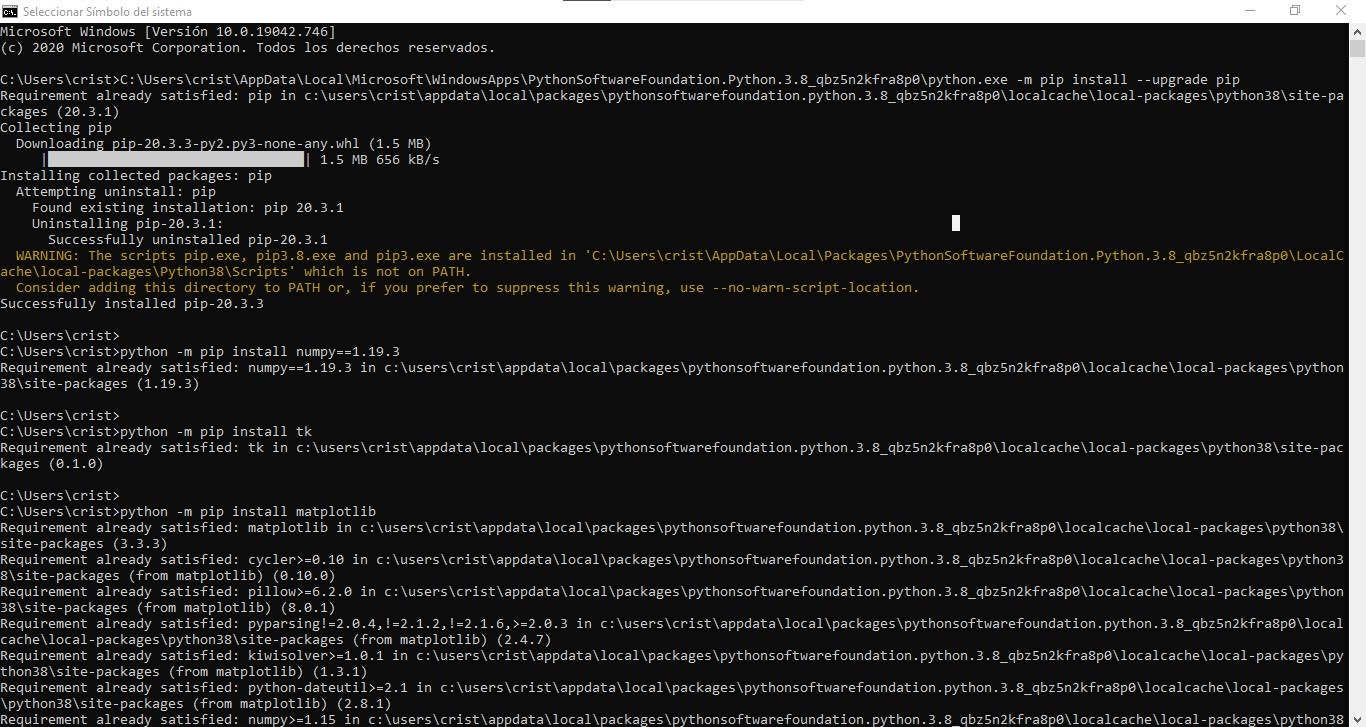
\includegraphics[width=1\textwidth]{imagen5PC}
		\caption{Instalación de paquetes 1}
	\end{figure}
	\begin{figure}[H]
		\centering
		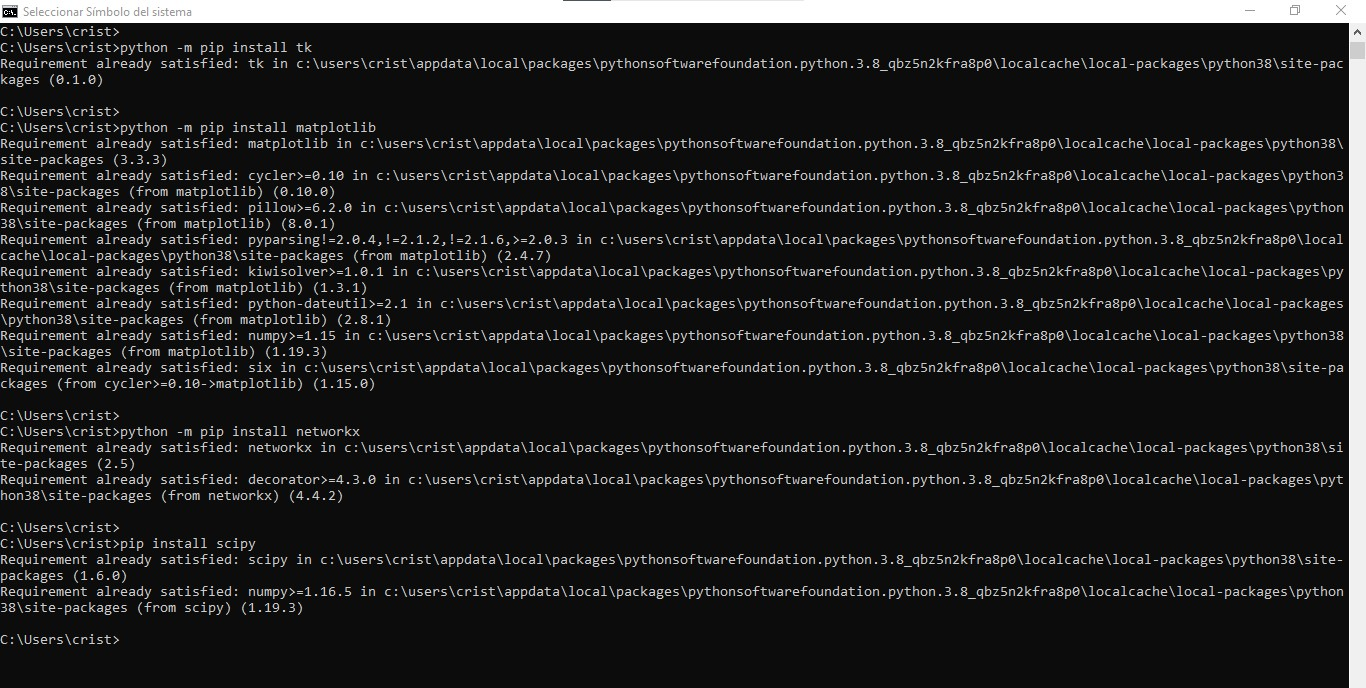
\includegraphics[width=1\textwidth]{imagen6PC}
		\caption{Instalación de paquetes 2}
	\end{figure}
\clearpage
	\section{Ejemplo de funcionamiento del software}
	En este apartado, se presentan los 2 módulos principales que el software maneja: \textbf{simulación del juego de la vida} y \textbf{generación de atractores}.
	\subsection{Life}
	Inicialmente, agregamos unas cuantas células al universo de tamaño 100x100 y las guardamos en un archivo .npy. Para guardar este patrón celular, se da click en el botón "save".
	\begin{figure}[H]
		\centering
		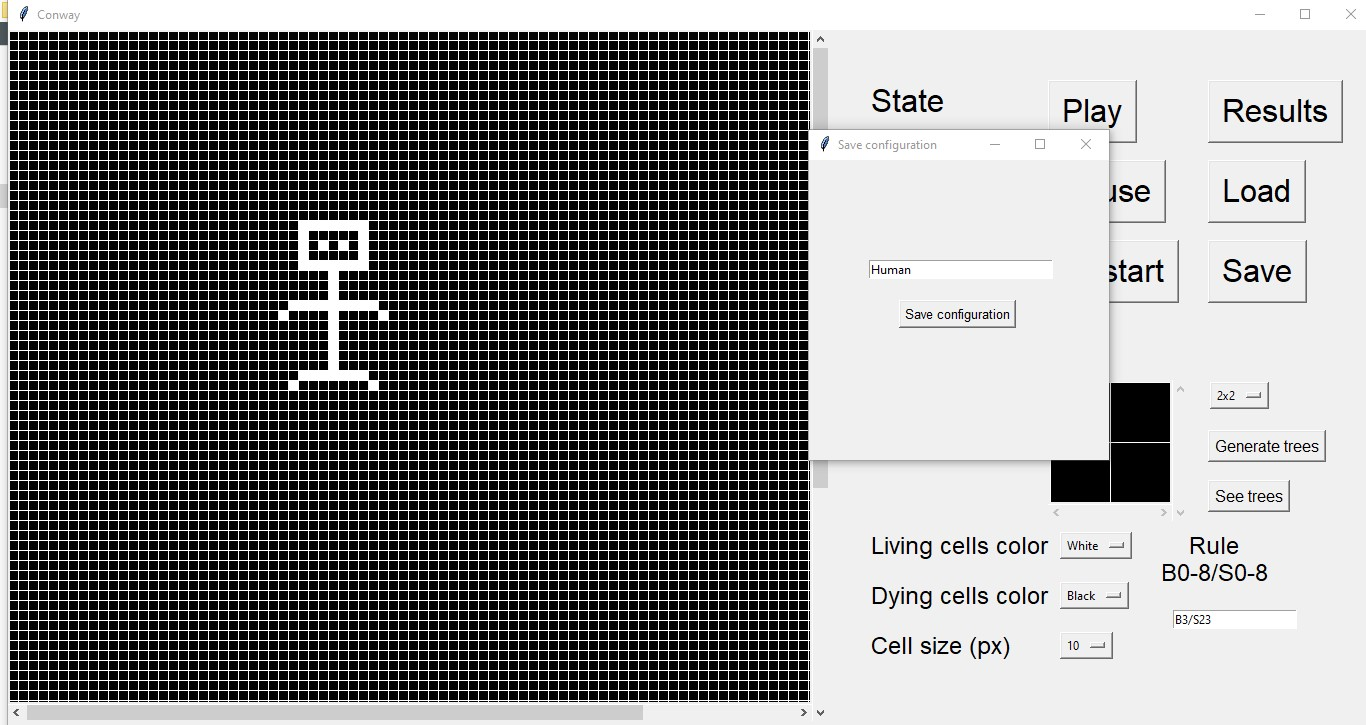
\includegraphics[width=1\textwidth]{imagen7PC}
		\caption{Las células vivas están de color blanco}
	\end{figure}
	\begin{figure}[H]
		\centering
		
\includegraphics[width=1\textwidth]{imagen8PC}
		\caption{Archivo generado llamado 'Human'}
	\end{figure}
	Al aplicar las reglas del juego de la vida (dar click en el botón "Play" para iniciar al juego de la vida), el patrón inicial 'Human.py' permanece por la eternidad en la siguiente figura celular:
	\begin{figure}[H]
		\centering
		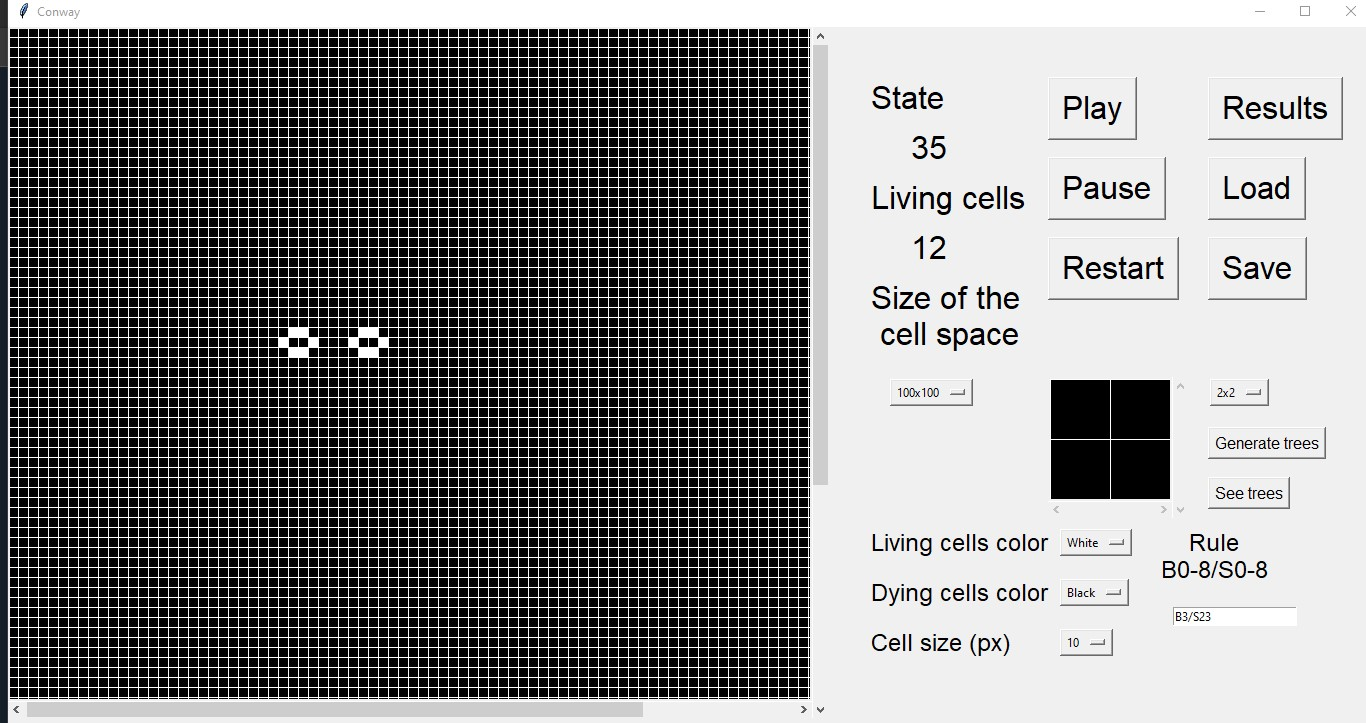
\includegraphics[width=1\textwidth]{imagen9PC}
		\caption{Patrón estático}
	\end{figure}
	El comportamiento de este patrón se puede verificar en la siguiente gráfica, que contiene la información de la relación 'célulasVivas-estado'. Esta gráfica se consigue dando click en el botón "Results"
	\begin{figure}[H]
		\centering
		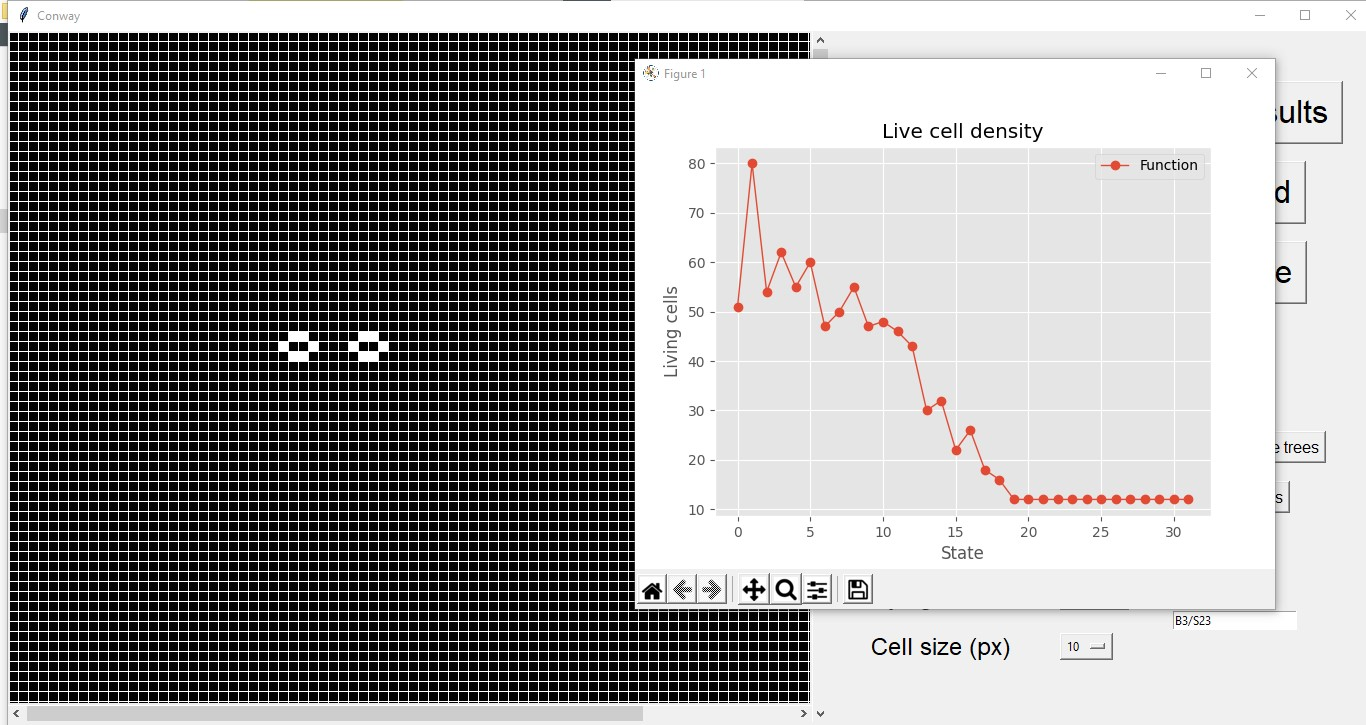
\includegraphics[width=1\textwidth]{imagen10PC}
		\caption{Células vivas por estado}
	\end{figure}

	Ahora, podemos cargar el patrón de células que se formó inicialmente dando click en el botón "Load".
	\begin{figure}[H]
		\centering
		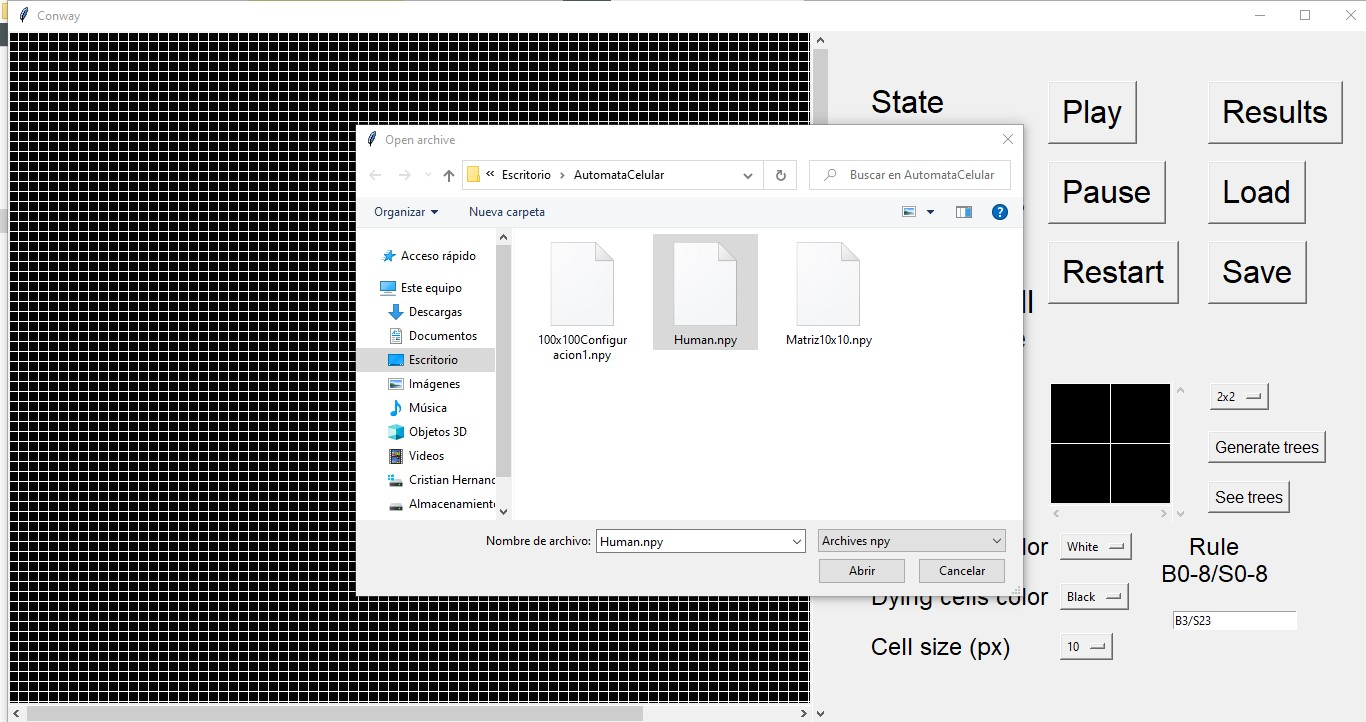
\includegraphics[width=1\textwidth]{imagen11PC}
		\caption{Cargar patrón}
	\end{figure}  
	\begin{figure}[H]
		\centering
		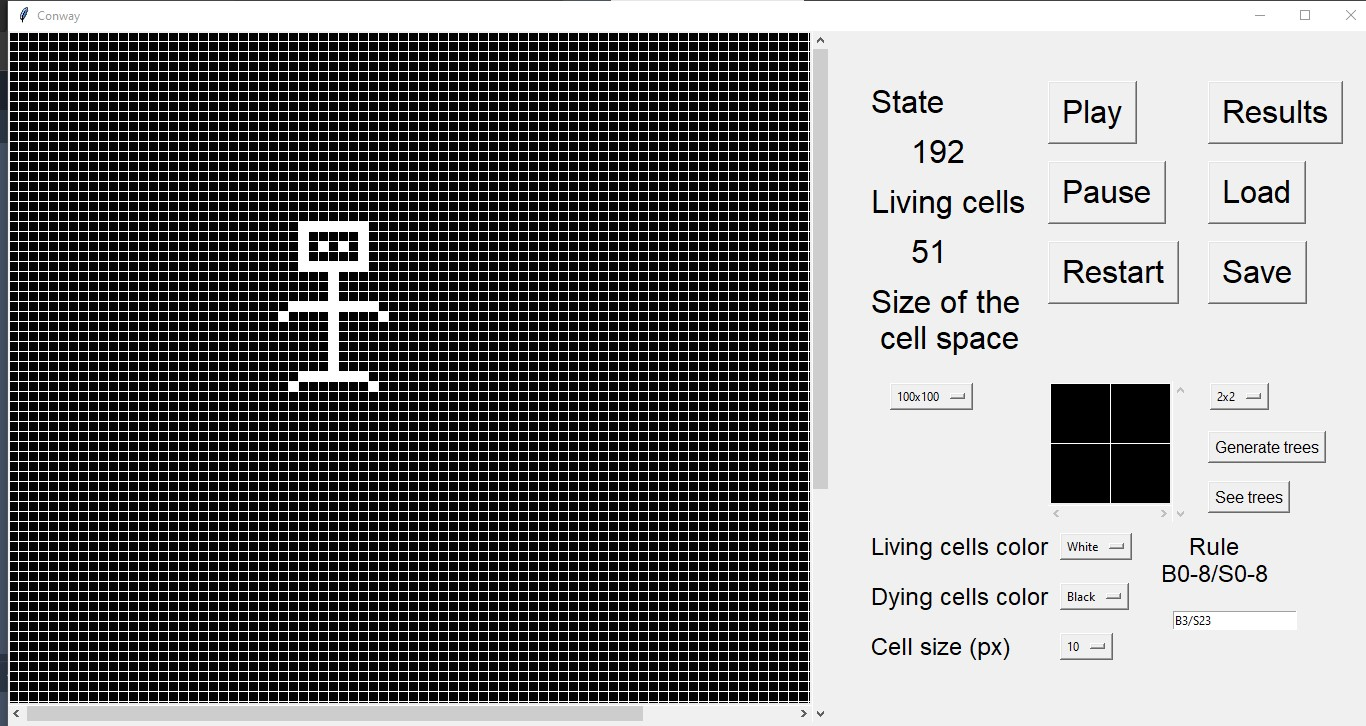
\includegraphics[width=1\textwidth]{imagen12PC}
		\caption{Patrón celular cargado}
	\end{figure} 

	\subsection{Generación de atractores}
	Un atractor es un punto, curva u otra figura que tiene como característica que un sistema, en el largo plazo, evoluciona hacia él; este atractor puede estar en universos planos de 2x2,3x3,4x4 y 5x5, el cual, en este caso, será hallado aplicando las siguientes reglas:
	
	\begin{itemize}
		\item \textbf{B3/S23}
		\item \textbf{B2/S7}
	\end{itemize}
	Los atractores son representados mediante grafos, los cuales son generados por las funciones del paquete Networkx de python (para el caso del universo plano de 2x2) y utilizando el software llamado 'Mathematica' (para los universos planos 3x3, 4x4 y 5x5). El programa genera todos los datos necesarios y los guarda en un archivo .txt para que Mathematica pueda ocuparlos para realizar los grafos. Cuando se da click en el botón "Generate trees", generamos los atractores. \\\\
	\textbf{¿Cómo se generan los atractores en el programa?}
	\\\\
	La idea principal de formar los nodos que pueden ir al atractor es la siguiente: \textit{en un universo plano mxm, se establecen $2^{mxm}$ patrones celulares, siendo estos regidos por las reglas del juego de la vida}. Un ejemplo para el lector, es el siguiente:
	\begin{figure}[H]
	\centering
	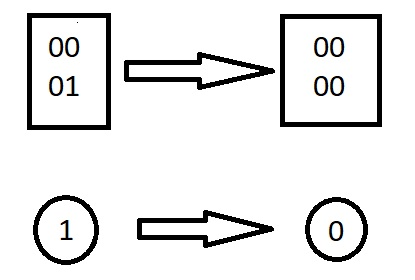
\includegraphics[width=0.6\textwidth]{GENACT}
	\caption{Arriba, en el universo celular 2x2, el patrón celular 0001 (en el estado 0) pasando a ser el patrón celular 0000 (en el estado 1). Abajo, la representación de ambos patrones celulares en números decimales dentro de nodos}
\end{figure}

Si se encuentra en algun estado del juego de la vida un patrón celular que ya había estado, se pasa al siguiente patrón celular, que en este caso, sería 0010.\\\\
De esta manera, el programa forma los nodos y nodos atractores. El programa los grafica para poder visualizar quienes son los diagramas de ciclos, para que después puedan ser clasificados y determinar si el sistema es caótico o complejo.
\clearpage
	\textbf{Atractores en el universo 2x2 plano}
	\\\\
	En las siguiente figuras, se pueden apreciar los atractores que existen en el universo celular 2x2 plano y a qué número decimal pertenece cada uno de ellos. Los atractores que existen aquí son los siguientes para la regla B3/S23: 0 y 15; mientras que para la regla B2/S7, los atractores en el mismo universo son: 0,12,10,9,6,5 y 3.
\begin{figure}[H]
	\centering
	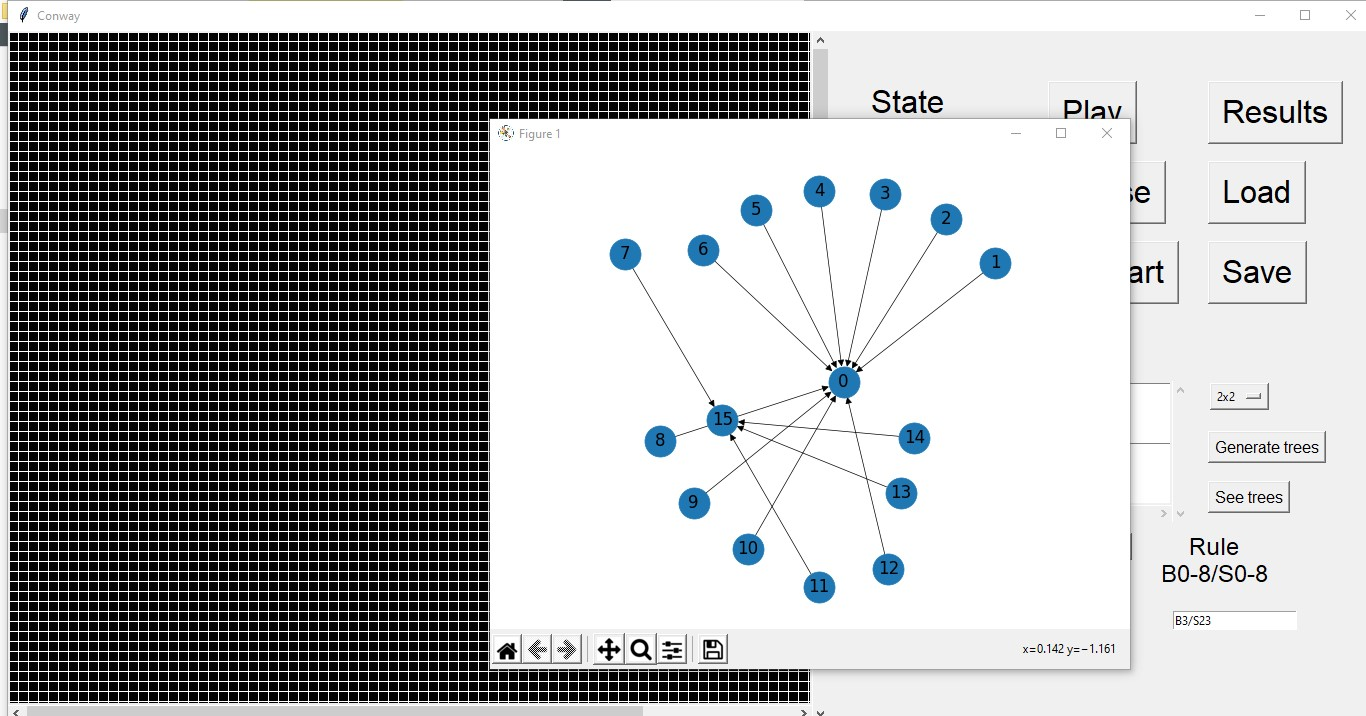
\includegraphics[width=0.9\textwidth]{imagen13PC}
	\caption{Vista de los atractores en el universo plano 2x2 con la regla B3/S23}
\end{figure}
\begin{figure}[H]
	\centering
	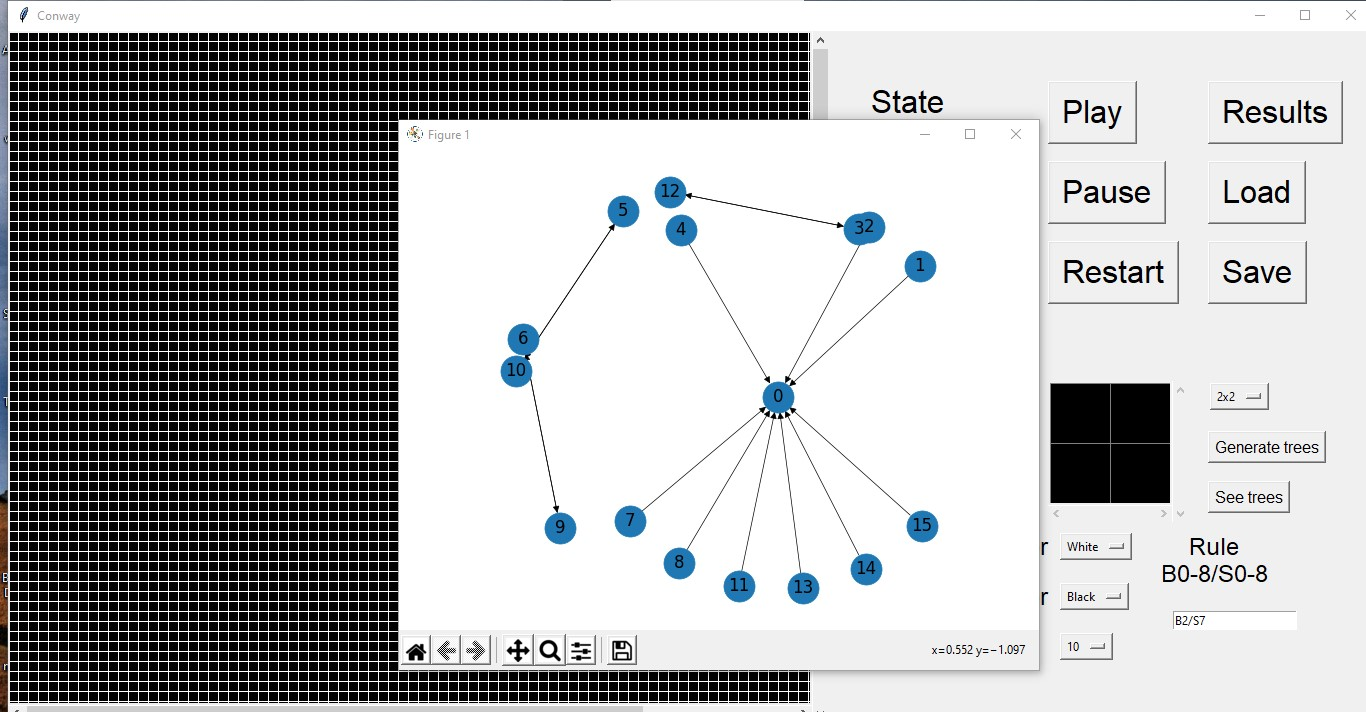
\includegraphics[width=0.9\textwidth]{imagen14PC}
	\caption{Vista de los atractores en el universo plano 2x2 con la regla B2/S7}
\end{figure} 
	\textbf{Atractores en el universo 3x3 plano}
	\\\\
	En las siguiente figuras, se pueden apreciar los atractores que existen en el universo celular 3x3 plano.
	\begin{figure}[H]
		\centering
		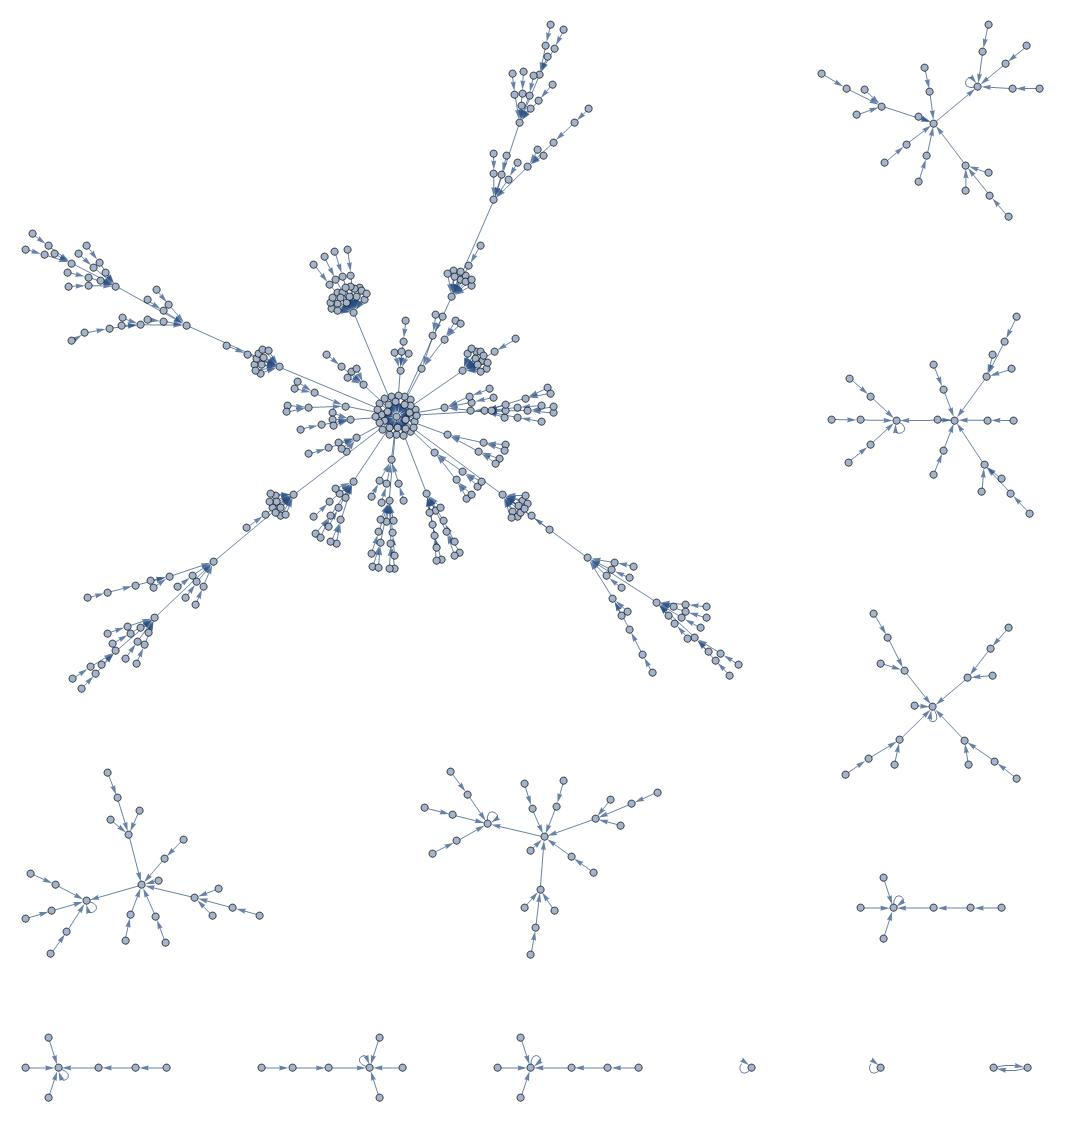
\includegraphics[width=0.9\textwidth]{imagen17PC}
		\caption{Vista de los atractores del universo plano 3x3 con la regla B3/S23}
	\end{figure}
\begin{figure}[H]
	\centering
	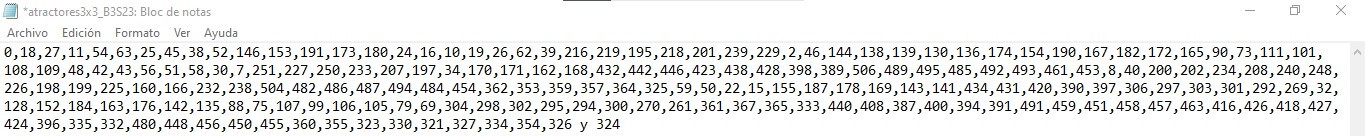
\includegraphics[width=0.9\textwidth]{imagen18PC}
	\caption{Atractores etiquetados del universo plano 3x3 con la regla B3/S23}
\end{figure}
\begin{figure}[H]
	\centering
	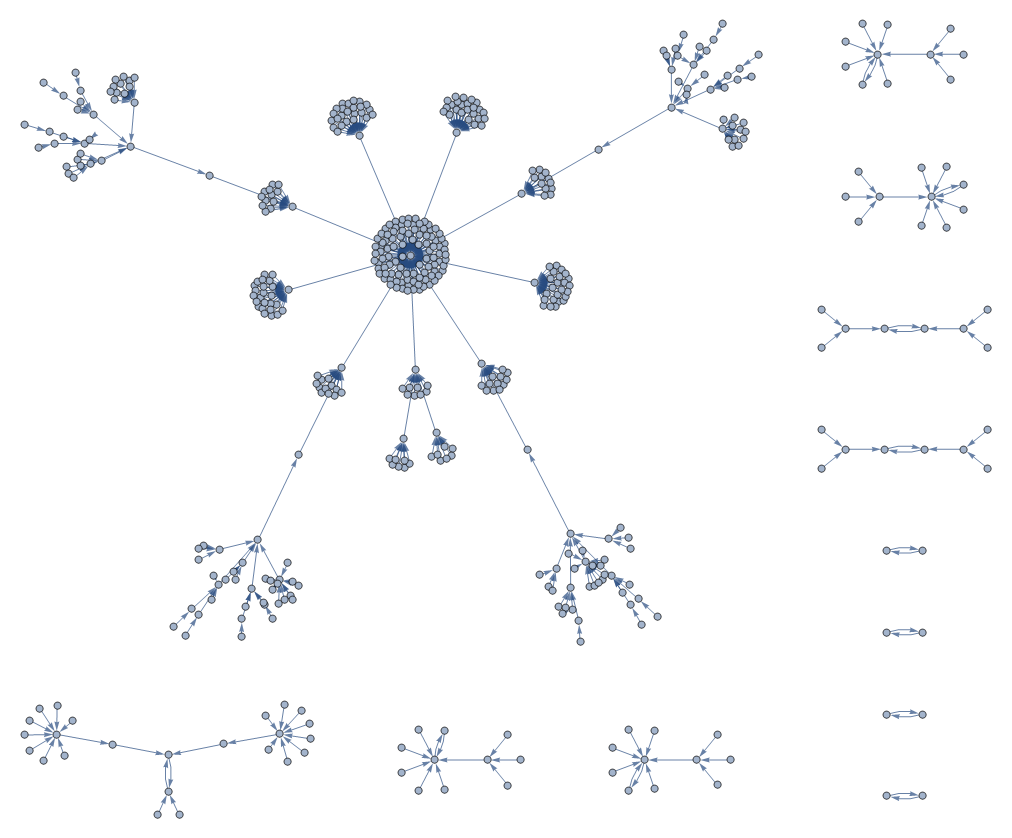
\includegraphics[width=0.9\textwidth]{imagen19PC}
	\caption{Vista de los atractores del universo plano 3x3 con la regla B2/S7}
\end{figure}
\begin{figure}[H]
	\centering
	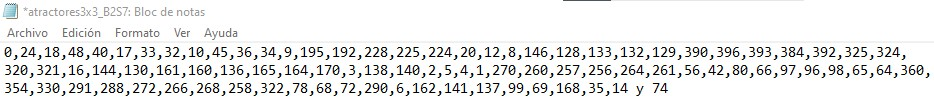
\includegraphics[width=0.9\textwidth]{imagen20PC}
	\caption{Atractores etiquetados del universo plano 3x3 con la regla B2/S7}
\end{figure}
\textbf{Atractores en el universo 4x4 plano}
\\\\
En las siguiente figuras, se pueden apreciar los atractores que existen en el universo celular 4x4. Por la cantidad de nodos mostrados, se complica la visualización de los atractores.
\begin{figure}[H]
	\centering
	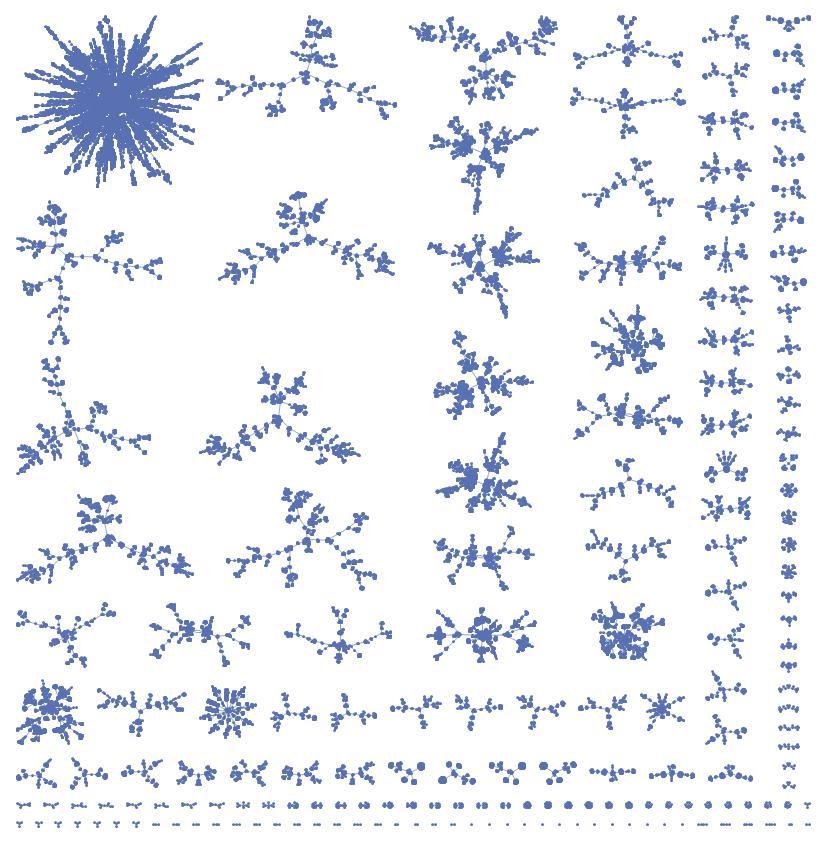
\includegraphics[width=0.9\textwidth]{imagen21PC}
	\caption{Vista de los atractores del universo plano 4x4 con la regla B3/S23}
\end{figure}
\begin{figure}[H]
	\centering
	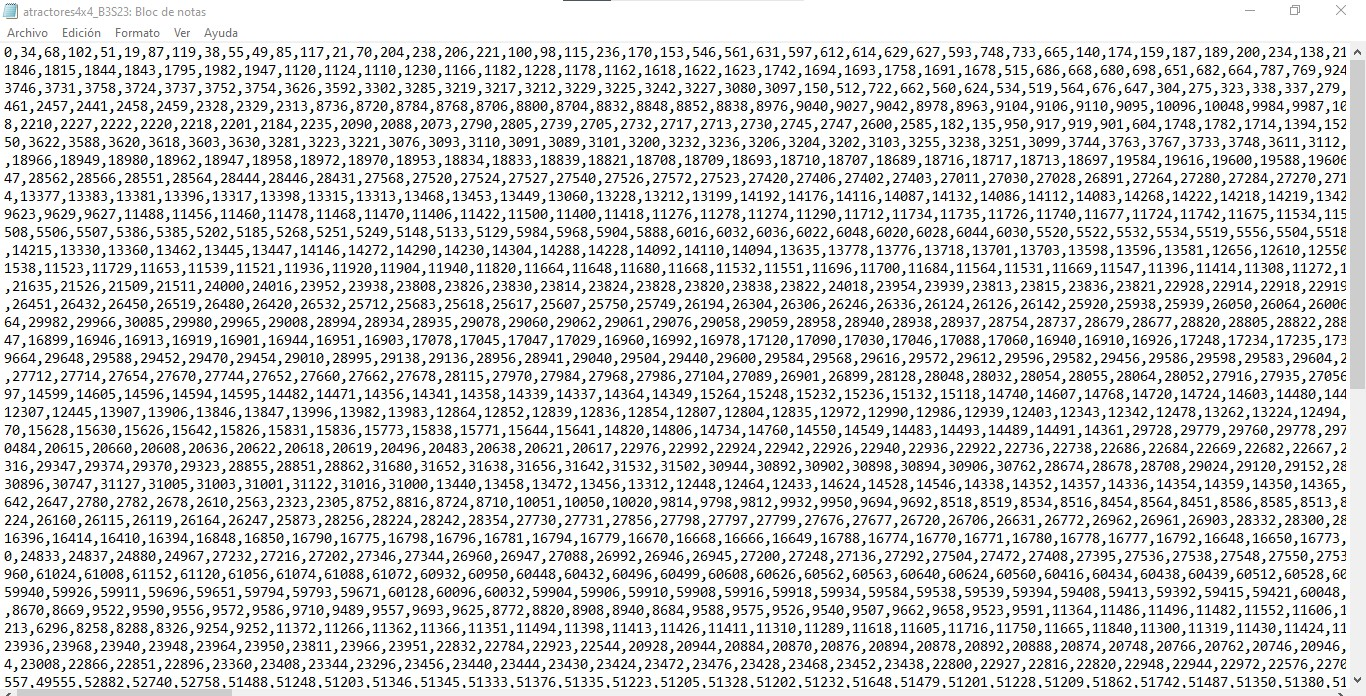
\includegraphics[width=0.9\textwidth]{imagen22PC}
	\caption{Algunos atractores etiquetados del universo plano 4x4 con la regla B3/S23}
\end{figure}
\begin{figure}[H]
	\centering
	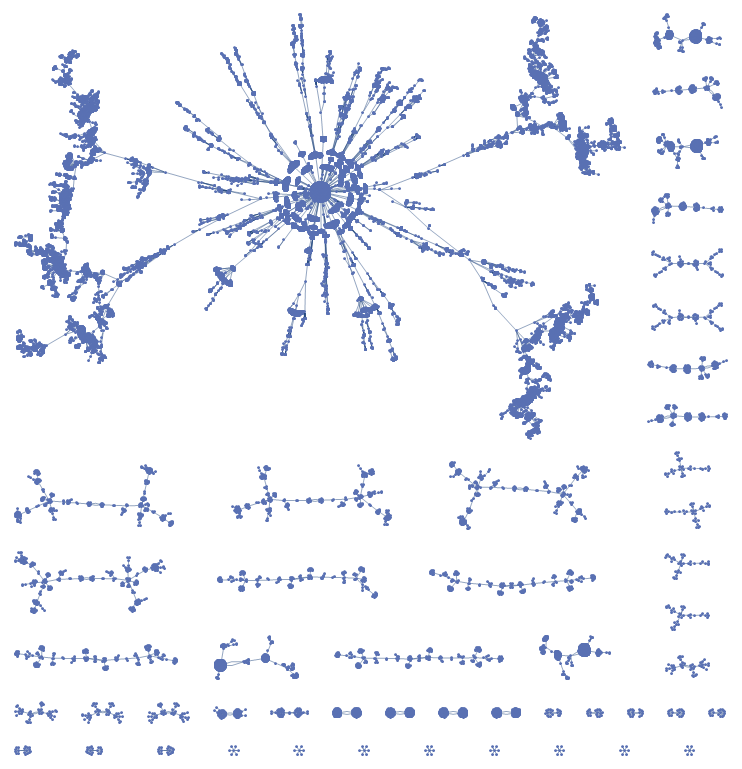
\includegraphics[width=0.9\textwidth]{imagen23PC}
	\caption{Vista de los atractores del universo plano 4x4 con la regla B2/S7}
\end{figure}
\begin{figure}[H]
	\centering
	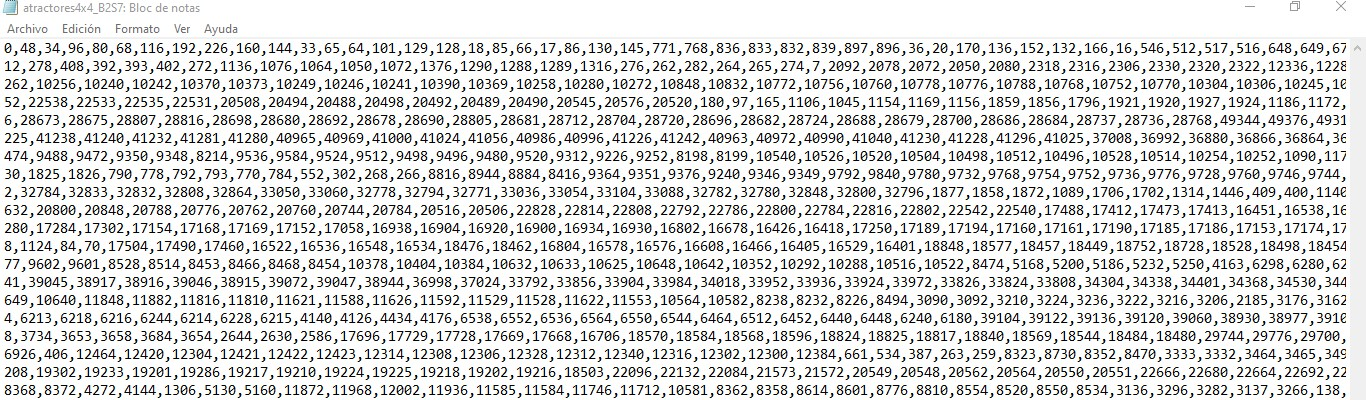
\includegraphics[width=0.9\textwidth]{imagen24PC}
	\caption{Algunos atractores etiquetados del universo plano 4x4 con la regla B2/S7}
\end{figure}

\subsection{Clasificación de los atractores}
Tomando en cuenta la clasificación Wolfram, los atractores generados en el programa (con las reglas B3/S23 y B2/S7) pertenecen a la clase IV (comportamientos complejos).
	\section{Código fuente}
	
	\inputminted{python}{Life9.py}
	
	
	\chapter{Conclusiones}
	En este momento, se tiene un juego de la vida en nuestras manos. Los resultados que pueden obtenerse con
	unas simples reglas son fantásticas, sin embargo, nos dirijimos a la pregunta: \textbf{¿es el juego de la vida un sistema caótico o complejo?}. La respuesta a esta pregunta se basa en los atractores generados por el software. Estos atractores tienen nodos relativamente idénticos a su cercanía, además, es complicado analizar la evolución dinámica de cada uno de los nodos, siendo que estos pueden ser atractores o pueden ser nodos atractores que apuntan a otros atractores. \\\\
	Hace ya bastante tiempo que se demostró que el juego de la vida es equivalente a una máquina universal de
	Turing, lo que le permitiría, teóricamente, realizar cualquier computación posible si se dispusiera de suficiente
	tiempo y suficiente memoria, por ejemplo, videojuegos de consolas de novena generación.\\\\
	Entre otras aplicaciones también estan las simulaciones de ciertos procesos químicos o incluso biológicos,
	tales como la formación de los patrones en la piel, el pelo o las conchas de ciertos animales. En las plantas
	sucede otro tanto: el comportamiento de los estomas (células de la epidermis de las hojas) es relativamente fácil
	de simular con unas pocas reglas. Con algo más de complejidad se puede simular también el funcionamiento
	de las neuronas, creando modelos que pese a su simplicidad acaban mostrando una extraordinaria complejidad
	cuando se les aplican ciertos patrones o valores iniciales.
	En el fondo, esa es la grandeza del comportamiento tanto del juego de la vida como de otros autómatas
	celulares: que de algo tan simple pueda surgir algo elaborado y complejo. Tan elaborado y tan complejo que
	todavía hoy en día se siguen estudiando.
	\chapter{Referencias}
	\begin{enumerate}
		\item http://www.ddlab.com/downloads/papers/2011\_b-of-a\_spanish.pdf
		\item https://www.eumed.net/libros-gratis/2011e/1100/atractor.html
		\item http://www.scielo.org.mx/scielo.php?script=sci\_arttext\&pid=S2448-66552019000200179
		\item http://delta.cs.cinvestav.mx/\textasciitilde{}mcintosh/oldweb/tesis/genaro/node5.html
		\item http://delta.cs.cinvestav.mx/\textasciitilde{}mcintosh/oldweb/s1997/todos/node16.html
	\end{enumerate}
	%http://juancespedes.es/blog/85/como-escapar-caracteres-especiales-en-latex
	%http://delta.cs.cinvestav.mx/\textasciitilde{}mcintosh/oldweb/tesis/genaro/node5.html
	%http://delta.cs.cinvestav.mx/~mcintosh/oldweb/s1997/todos/node16.html
\end{document}
%\maketitle%%esta linea de codigo coloca la siguiente estructura: titulo, autor y fecha actual del sistema


